\section{Analysis of dependencies using Tareador}
\justify
In this section we are going to take a look at data dependencies of both algorithm using Tareador.
\subsection{Tareador analysis of Jacobi approach}
\justify
First of all we worked with Jacobi algorithm. Given a first execution using tareador we got the following dependency graph.

\begin{figure}[h!]
    \centering
    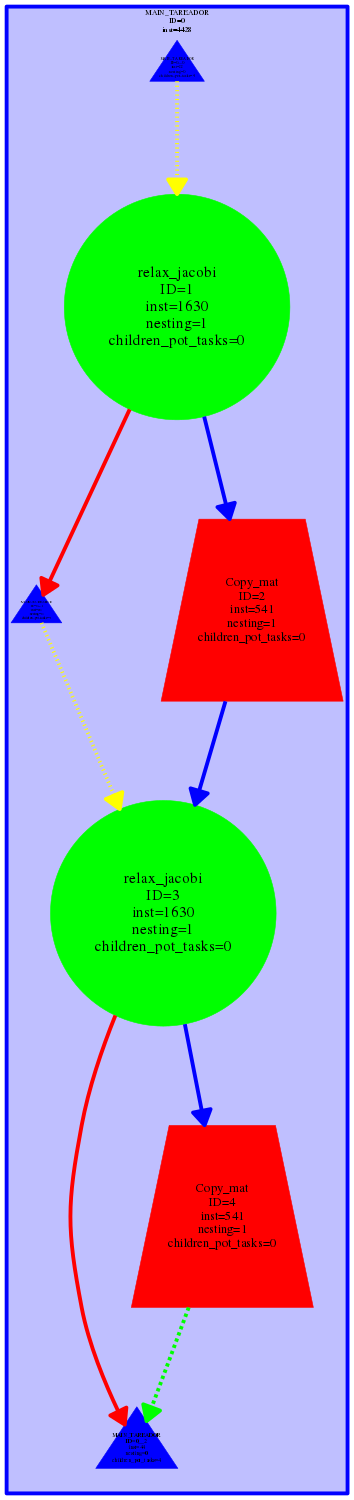
\includegraphics[width=0.15\textwidth]{jacoby_tareador.png}
    \caption{Jacobi Tareador default execution.}
    \label{fig:jacobitar}
\end{figure}

\justify
As you can see in the following image the code generated is sequential and there is much nothing we can do, as we have dependencies between the calls and copy mat. If we go for a more finner granularity to one task for the most inner loop of the algorithm we can observe the following.

\justify
You can assume that red spots are inner loop iterations. These are secuentially ordered because of data dependencies. Specially the dependencies are in the sum variable, this can be easily solved with a reduction. The other variable that causes serialization is the diff variable. You will see our approach in the next section. 

\begin{figure}[H]
    \centering
    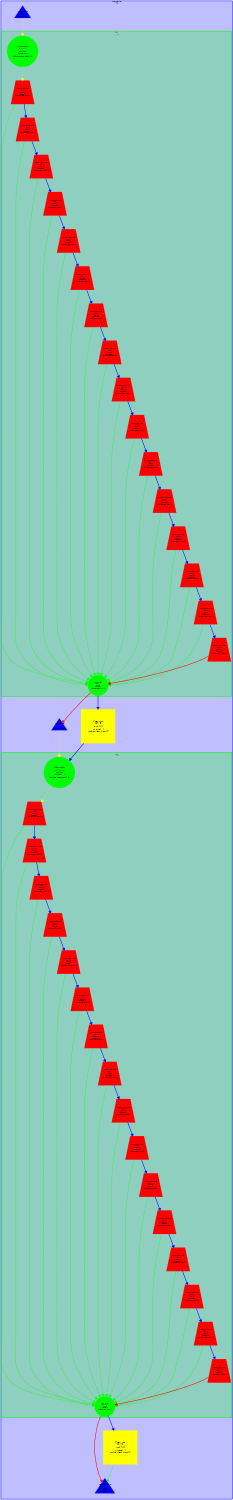
\includegraphics[width=0.12\textwidth]{jacoby_inner_tareador.png}
    \caption{Jacobi Tareador finer granularity execution.}
    \label{fig:jacobinnertar}
\end{figure}

\justify
Finally, we deactivated the variables in order to see if the graph generated there is possible parallelism or not.

\begin{figure}[H]
    \centering
    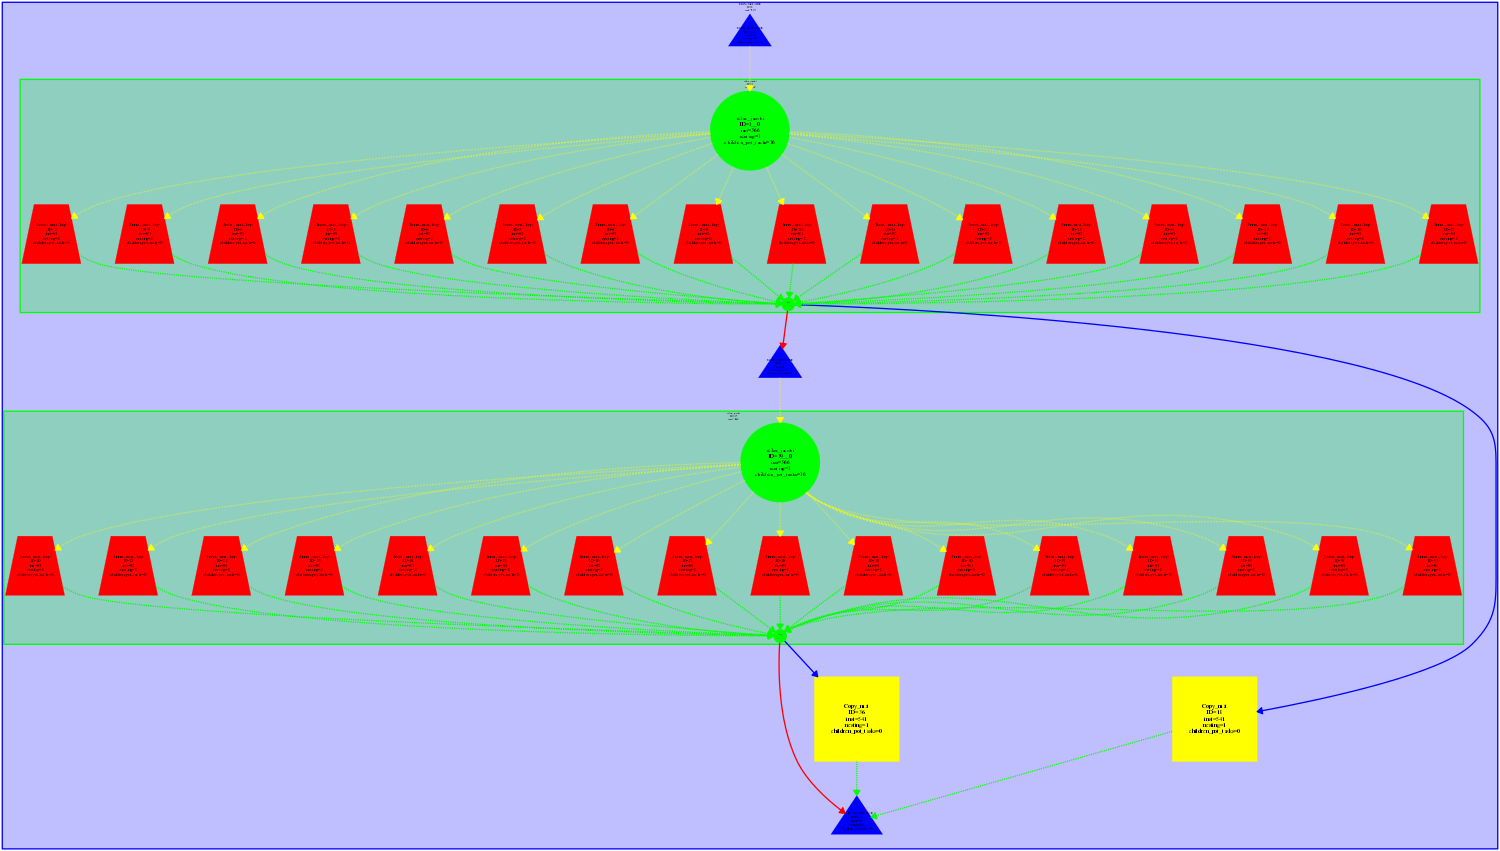
\includegraphics[width=0.75\textwidth]{jacoby_inner_nosumnou_tareador.png}
    \caption{Jacobi Tareador finer granularity execution with sum deactivated.}
    \label{fig:jacobinnertarnosum}
\end{figure}
\justify
As you can observe yes, the code has no dependencies between iterations. 

\subsection{Tareador analysis of Gauss-Seidel approach}
\justify
In this subsection we are going the repeat the analysis done with Jacobi's approach.

\justify
On a first execution with no granularity set, we obtain the following task graph.

\begin{figure}[H]
    \centering
    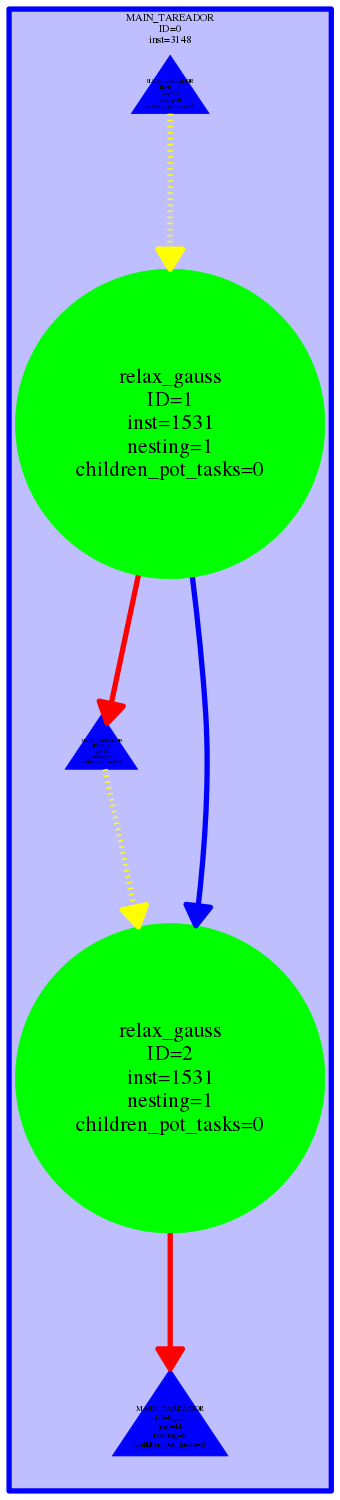
\includegraphics[width=0.15\textwidth]{gauss-tareador.png}
    \caption{Gauss-Seidel Tareador default execution.}
    \label{fig:gausstareador}
\end{figure}

\justify
As you can see from the last subsection we get similar graph with the difference that there is not \texttt{copy\_mat} between calls to the algorithm. In practice there is no actual difference as the dependencies due to the order of the code are still there, so we can not paralelize at that granularity. 
\justify
Going to inner-most loop granularity we get the following graph.

\begin{figure}[H]
    \centering
    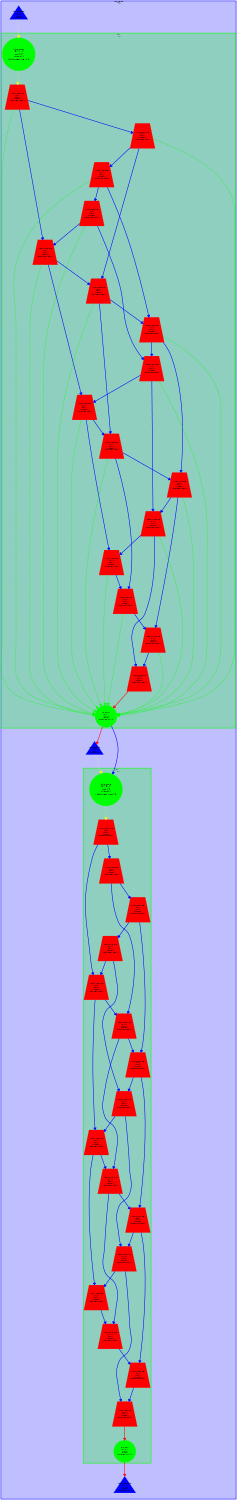
\includegraphics[width=0.11\textwidth]{gauss_inner-tareador.png}
    \caption{Gauss-Seidel Tareador finer granularity.}
    \label{fig:gaussfinne}
\end{figure}

\justify
In comparison the the Jacobi inner most loop granularity Tareador graphic you can observe that there appear more dependencies between tasks. We have the other dependencies, for sum and diff variables, but each iteration has dependencies with $(i-1,j)$ and $(i, j-1)$ elements of the matrix, being i and j the row and the column for the current block. 

\justify
Disabling the dependencies we obtain the following task graph.
\begin{figure}[H]
    \centering
    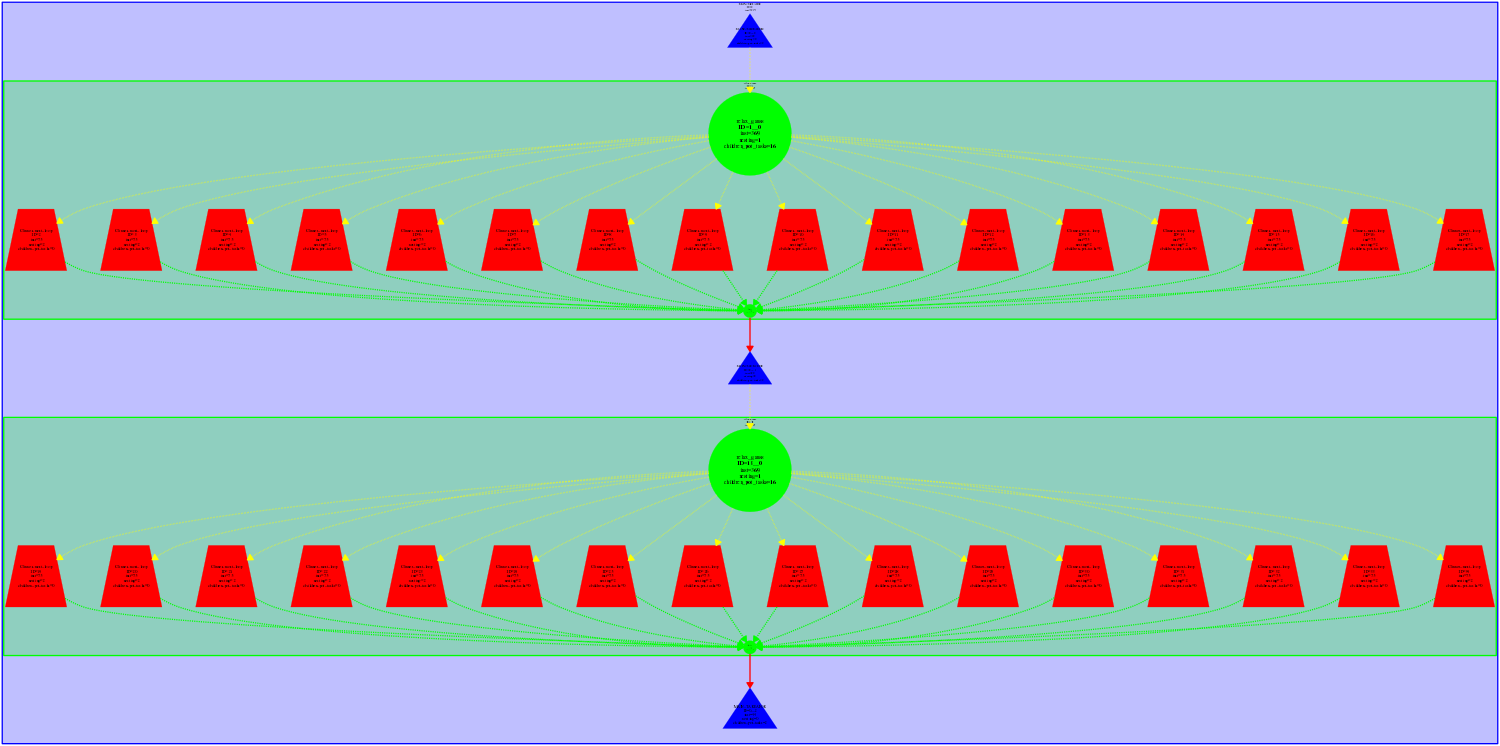
\includegraphics[width=0.63\textwidth]{gauss-inner-nosumnou-tareador.png}
    \caption{Gauss-Seidel Tareador finer granularity and deactivated dependencies.}
    \label{fig:gausstareadornosum}
\end{figure}
So we can also paralelize the Gaus-Seidel aproach taking into account the dependencies generated.